\documentclass{ctexart}
\title{ 深度学习实践 homework2}
\author{PB22061199 樊祉奕}
\date{\today}
\usepackage{subcaption}
\usepackage{ctex}
\usepackage{float}  
\newcommand\degree{^\circ}
\usepackage{graphicx}
\usepackage{pifont}
\usepackage{titlesec}
\usepackage{graphicx}
\usepackage{pifont}
\usepackage{setspace}
\usepackage{titlesec}
%\titlespacing{\section}{0pt}{\baselineskip}{\baselineskip}
%\singlespacing
\usepackage{amsmath}
\usepackage{geometry}
\usepackage{setspace}
\onehalfspacing
\geometry{a4paper,scale=0.8}
\usepackage{caption}
\usepackage{graphicx}
\usepackage{float} 
%\usepackage{subfigure}
\usepackage{subcaption}
\usepackage{placeins}
\usepackage{fancyhdr}
\pagestyle{fancy}
\usepackage{listings} %导入包
\usepackage[dvipsnames]{xcolor}

\fancyhf{}  % 清除所有页眉和页脚的设置
\fancyfoot[C]{\thepage}  % 页码显示在页脚中间
\ctexset{
	section={
		%format用于设置章节标题全局格式,作用域为标题和编号
		%字号为小三,字体为黑体,左对齐
		%+号表示在原有格式下附加格式命令
		format+ = \zihao{-3} \songti \raggedright,
		%name用于设置章节编号前后的词语
		%前、后词语用英文状态下,分开
		%如果没有前或后词语可以不填
		name = { , . },
		%number用于设置章节编号数字输出格式
		%\chinese输出section编号为中文,\arabic输出为阿拉伯数字
		number = \chinese{section},
		%beforeskip用于设置章节标题前的垂直间距
		%ex为当前字号下字母x的高度
		%基础高度为1.0ex,可以伸展到1.2ex,也可以收缩到0.8ex
		beforeskip = 1.0ex plus 0.2ex minus .2ex,
		%afterskip用于设置章节标题后的垂直间距
		afterskip = 1.0ex plus 0.2ex minus .2ex,
		%aftername用于控制编号和标题之间的格式
		%\hspace用于增加水平间距
		aftername = \hspace{0pt}
	},
	subsection={
		format+ = \zihao{4} \songti \raggedright,
		%仅输出subsection编号且为中文
		number = \arabic{subsection},
		name = {,.},
		beforeskip = 1.0ex plus 0.2ex minus .2ex,
		afterskip = 1.0ex plus 0.2ex minus .2ex,
		aftername = \hspace{0pt}
	},
	subsubsection={
		%设置对齐方式为居中对齐
		format+ = \zihao{-4} \songti ,
		%仅输出subsubsection编号,格式为阿拉伯数字,打字机字体
		number =\arabic{subsection}-\arabic{subsubsection},
		name = {,.},
		beforeskip = 1.0ex plus 0.2ex minus .2ex,
		afterskip = 1.0ex plus 0.2ex minus .2ex,
		aftername = \hspace{0pt}
	}
}
\begin{document}
\maketitle
\section{软件功能概述}
该软件实现了一个股票指数分析系统,包含以下功能:

\subsection{数据获取}
通过东方财富API获取股票指数数据,支持上证指数、深证成指和道琼斯指数的日线($Day\_Stock\_lookup.py$)和周线数据($week\_Stock_lookup.py$)。

\subsection{数据可视化}
使用mplfinance库绘制周线图、月线图($StockPlotter\_week.py$)及面积图($Otherplot.py$),支持显示开盘价、收盘价、成交量等指标。

\subsection{GUI交互}
软件基于Tkinter的图形界面($GUI\_achieve.py$),用户可选择国家、指数类型,输入日期或年份,触发查询或绘图操作。


系统整合了数据爬取、解析、存储与可视化功能,为股票指数分析提供一站式工具。
\begin{figure}[htbp]
	\centering
	\begin{minipage}{0.49\linewidth}
		\centering
		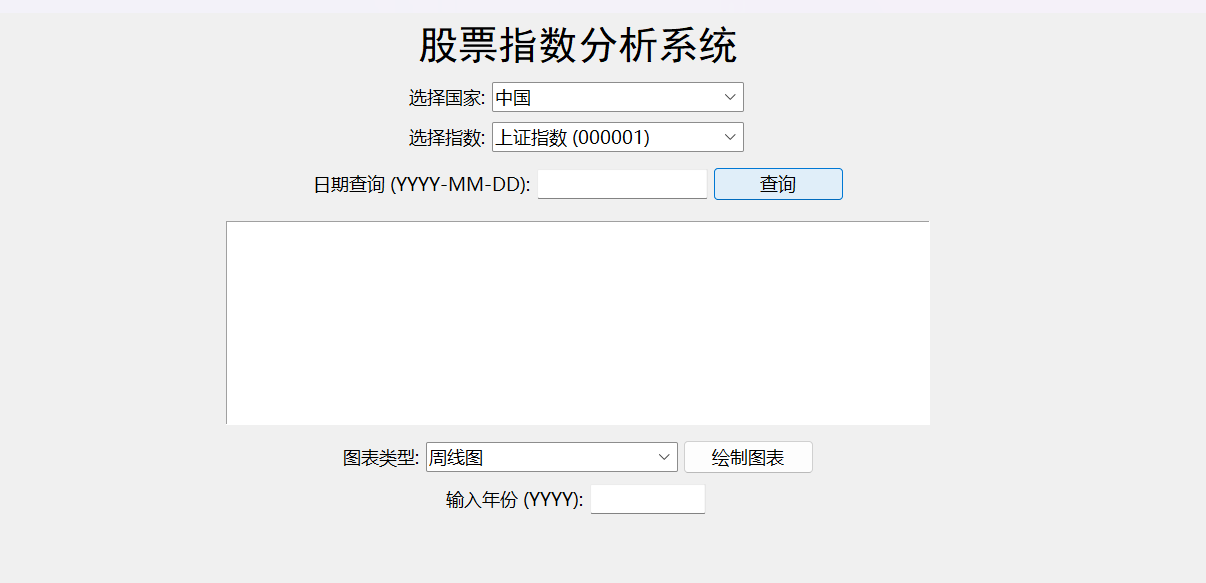
\includegraphics[width=0.9\linewidth]{demonstrations_ex.png}
		\caption{软件界面演示}
		\label{软件界面演示}%文中引用该图片代号
	\end{minipage}
	%\qquad
	\begin{minipage}{0.49\linewidth}
		\centering
		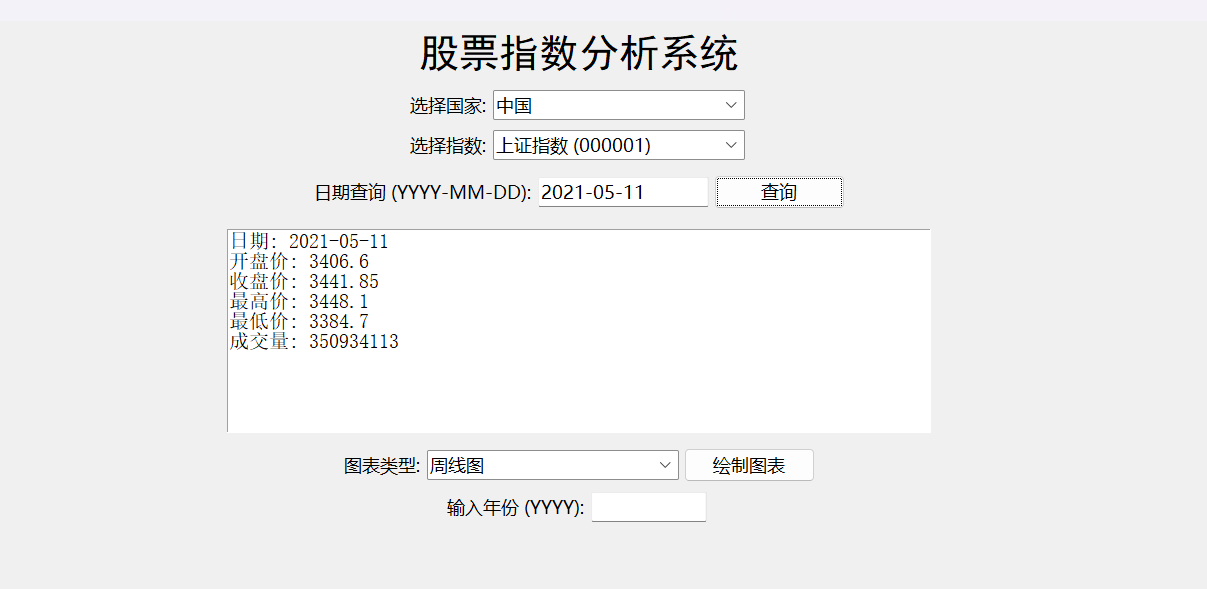
\includegraphics[width=0.9\linewidth]{daily_lookup.png}
		\caption{日数据查询}
		%\label{日数据查询}%文中引用该图片代号
	\end{minipage}
\end{figure}
\begin{figure}[htbp]
	\centering
	\begin{minipage}{0.49\linewidth}
		\centering
		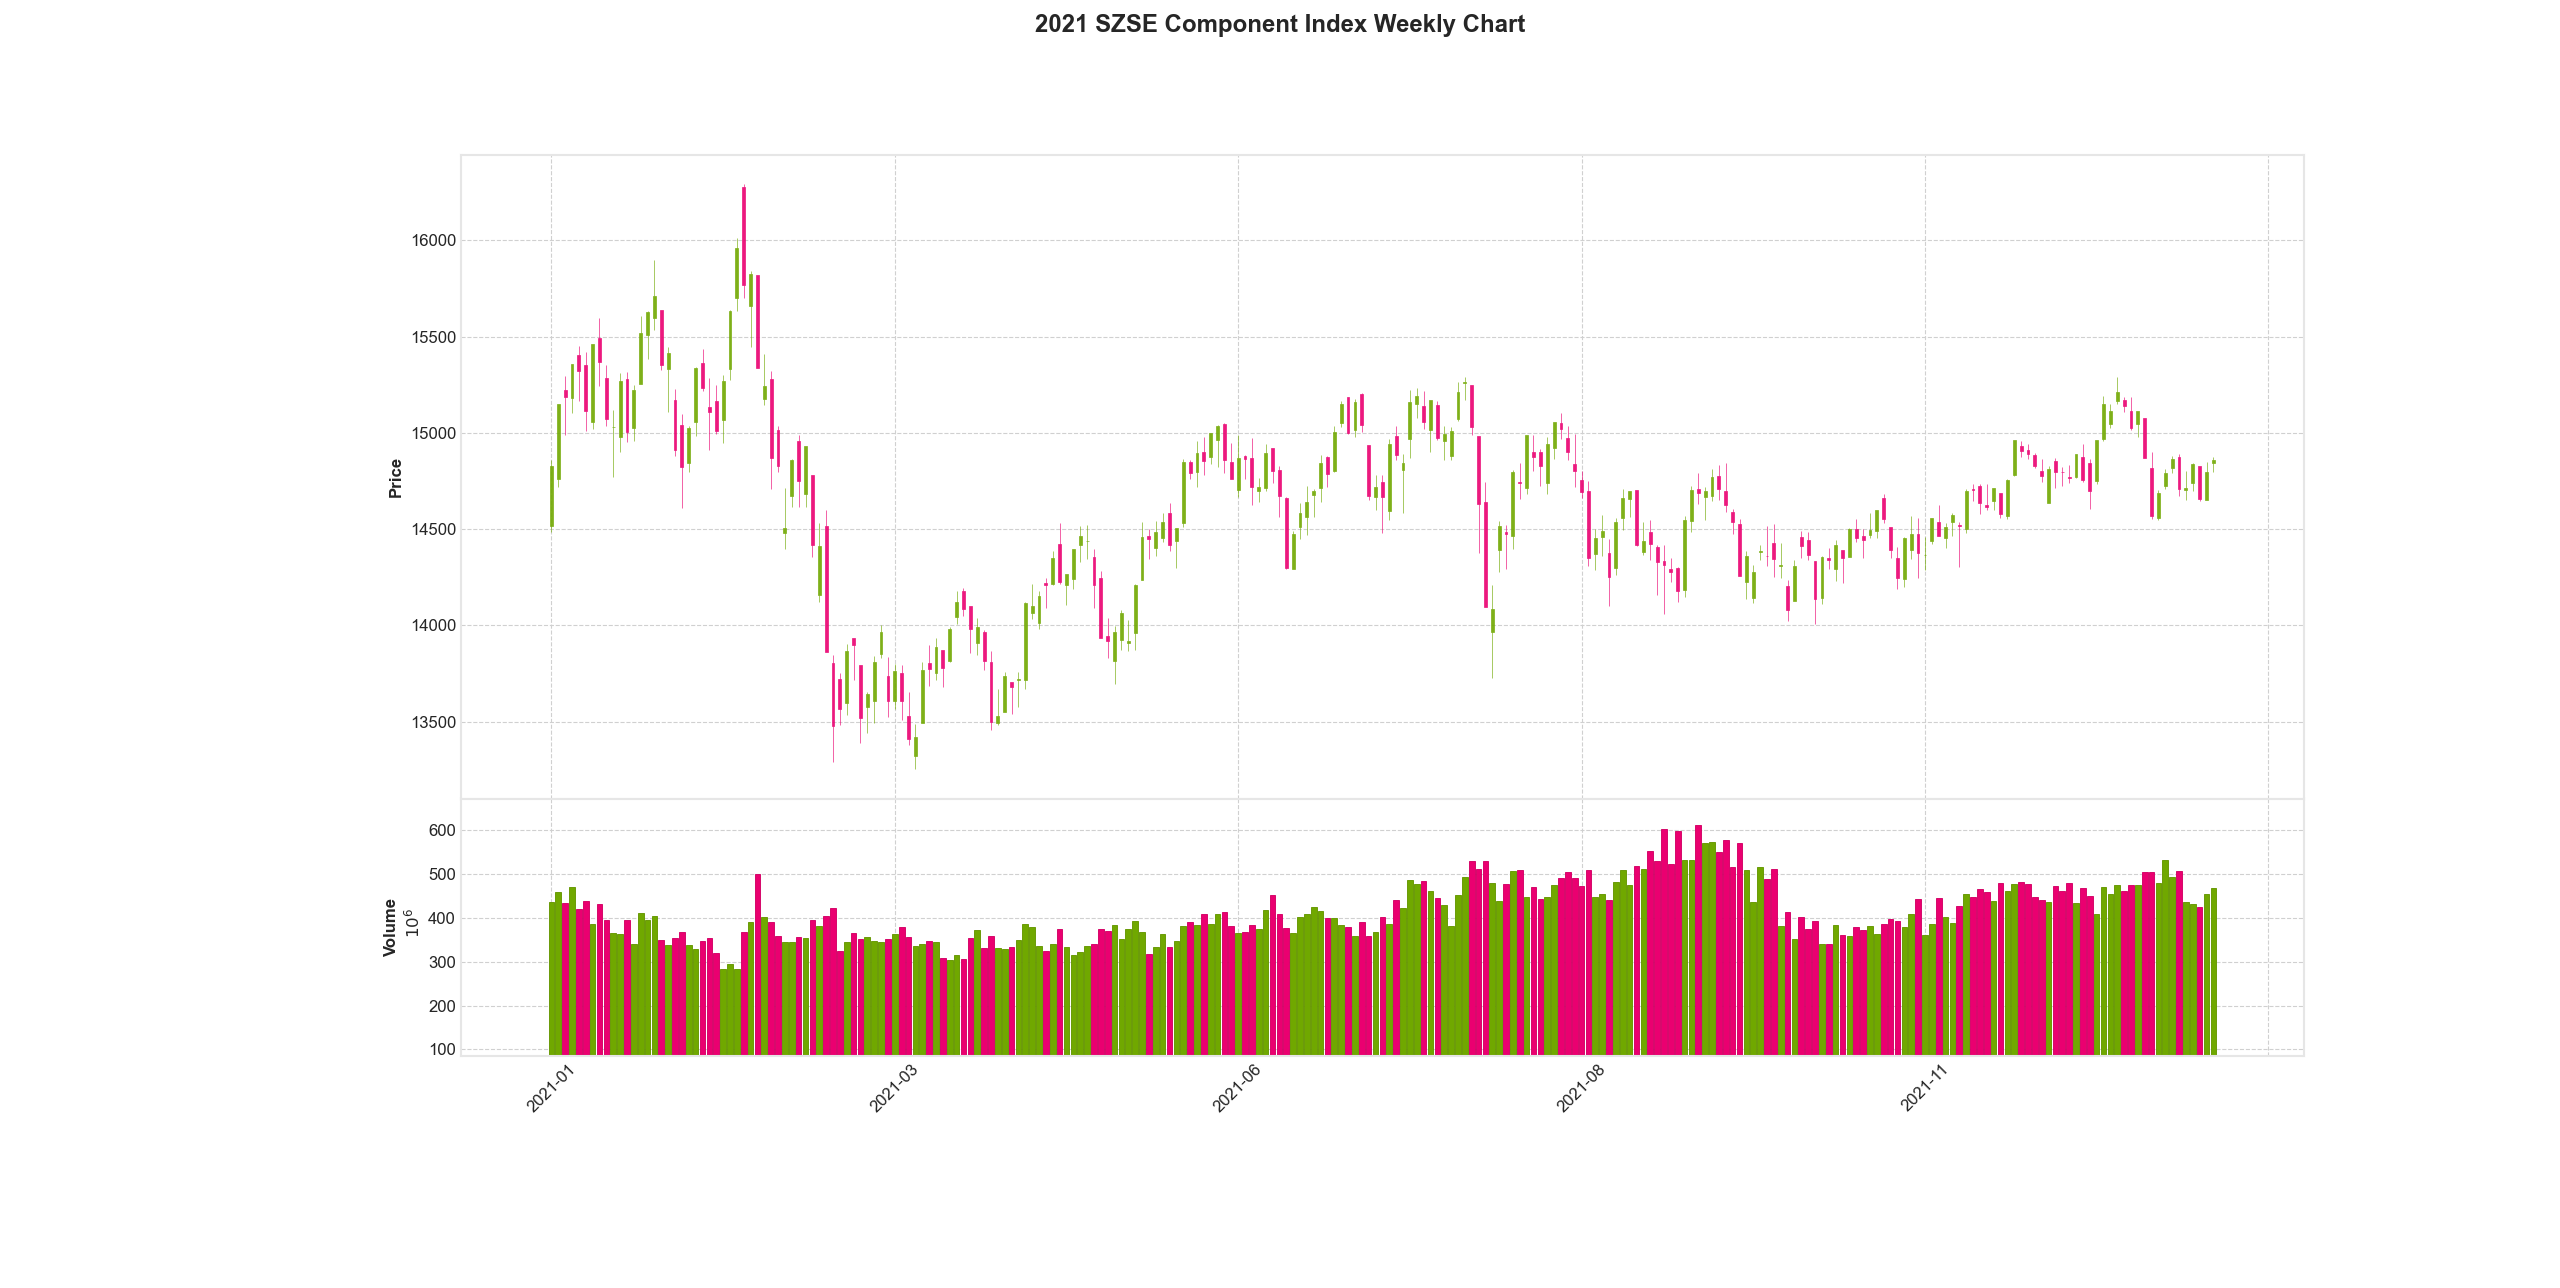
\includegraphics[width=0.9\linewidth]{weekly_chart.png}
		\caption{周线图}
		\label{周线图}%文中引用该图片代号
	\end{minipage}
	%\qquad
	\begin{minipage}{0.49\linewidth}
		\centering
		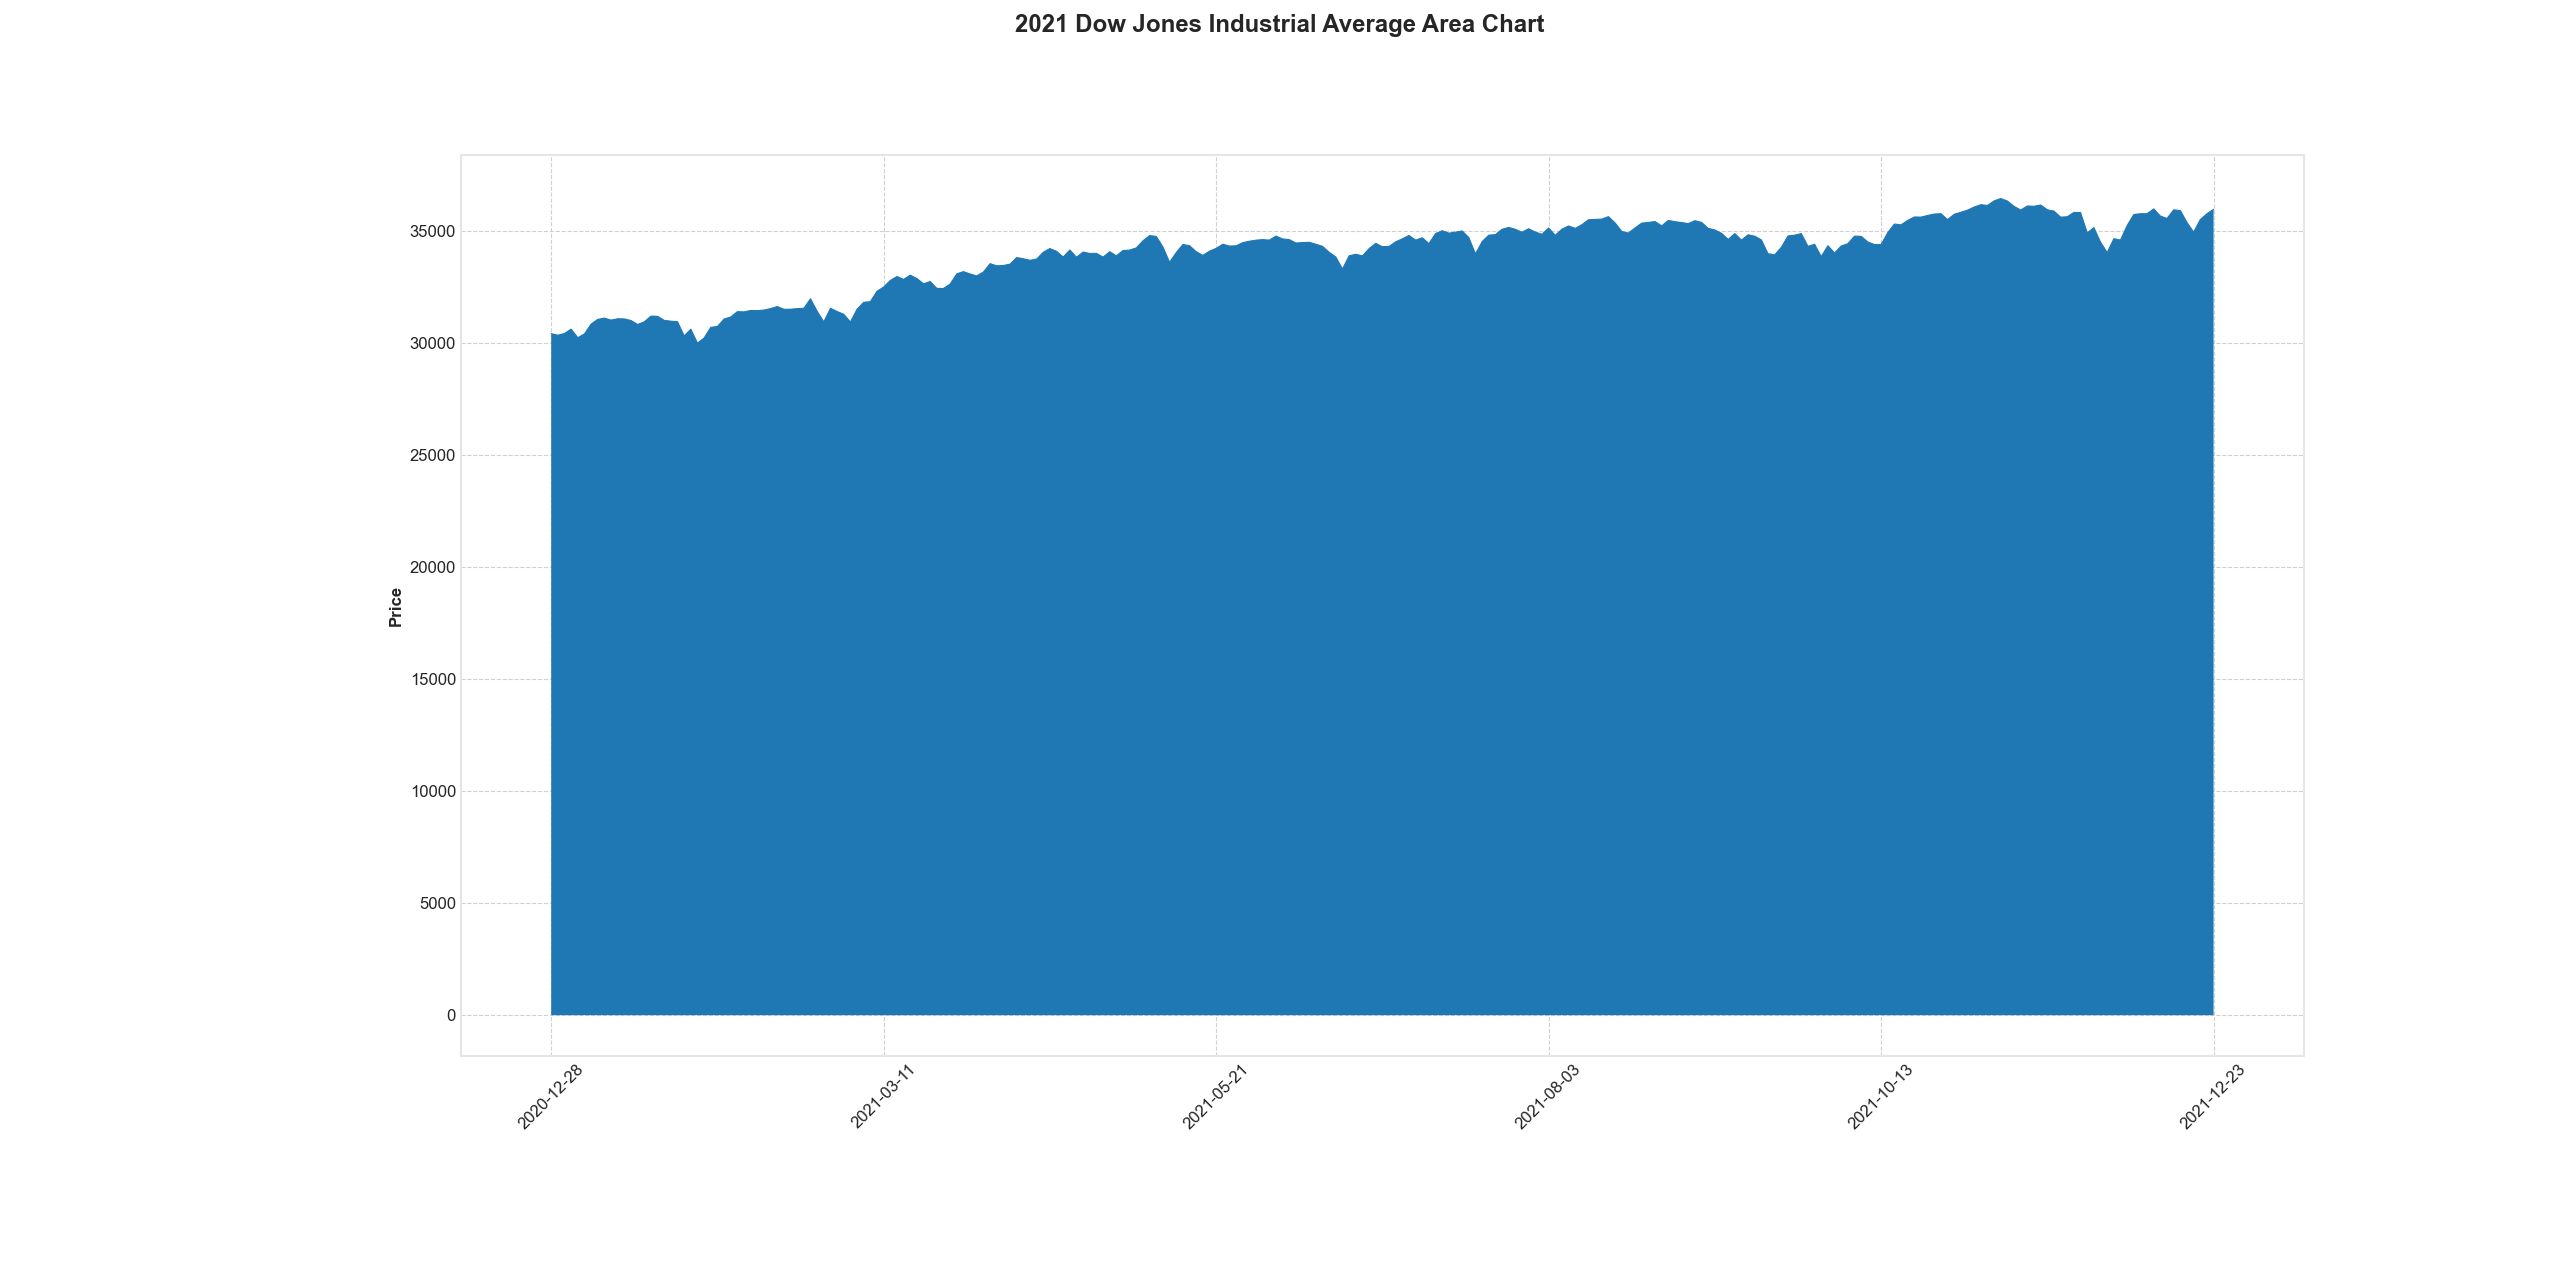
\includegraphics[width=0.9\linewidth]{area_chart.png}
		\caption{面积图}
		%\label{日数据查询}%文中引用该图片代号
	\end{minipage}
\end{figure}

\section{主要类}
\subsection{$class Day\_StockData$}

\subsubsection{功能}

\subsection{$class week\_StockData$}

\subsection{$class StockPlotter$}

\subsection{$class StockPlotter$}
\subsection{$StockGUI$}

\section{设计困难及解决方法}
\section{作业收获}


\end{document}